\chapter{Appendix}


%\begin{figure}[!ht]
%    \centering
%    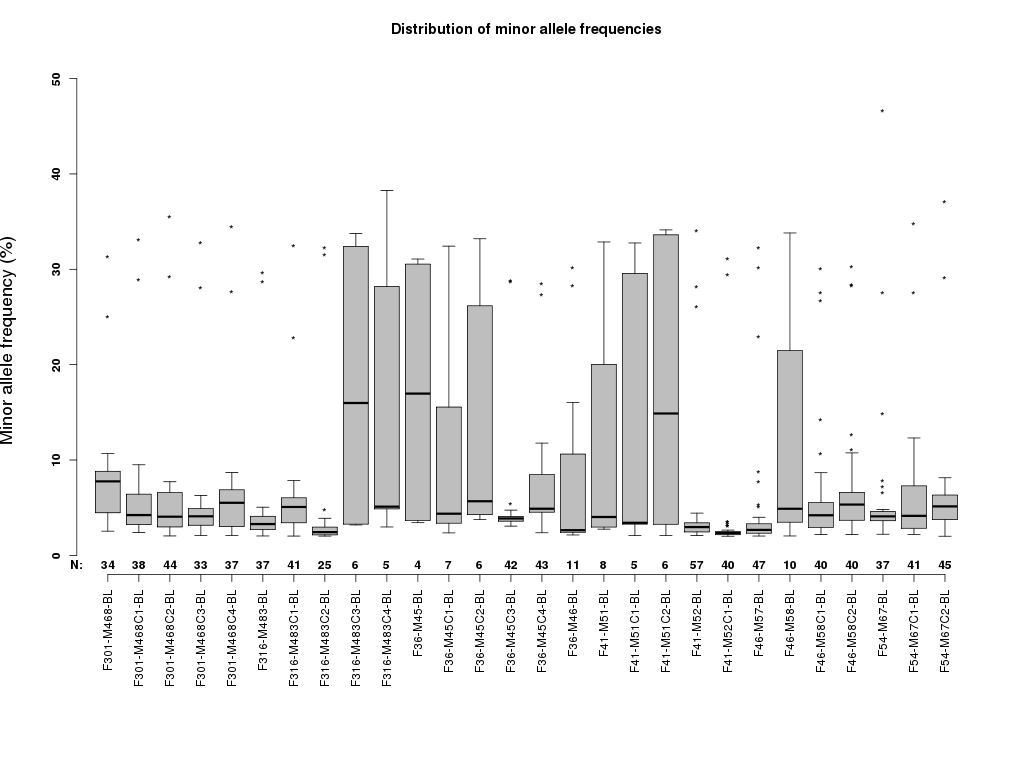
\includegraphics[width=1\textwidth]{images/galaxy-boxplot.png}
%    \caption[Galaxy Boxplot]{Galaxy Boxplot} 
%    \label{app:galaxy-boxplot}
%\end{figure}
The following listing represents the Pipeline for contamination detection defined in Cloudgene 
\begin{lstlisting}[caption={Cloudgene YAML file, defining the HaploChecker Workflow}, label=appyaml]

name: Contamination Check
description:  Check for Contamination
version: 0.1
website: 
category: mtDNA

cluster:

  image: us-east-1/ami-da0cf8b3
  type: m1.large,m1.xlarge
  ports: 80,50030,50070
  creationOnly: false
  installMapred: true
  initScript: install.sh
  service: hadoop
 
mapred:

  steps:
 
    - name: Create HaploGrep Inputfile
      jar: heteroplasmy-check-1.0.jar
      params: --input $input2 --output ${haplogrepInput}.txt

    - name: Haplogroup Contamination Check
      jar: haplogrep.jar
      params: --in ${haplogrepInput}.txt --out ${haplogroupsCheck}.txt --phylotree 16

    - name: Report Creation
      rmd: report.Rmd
      output: ${report}.html
      params: ${haplogroupsCheck}.txt

  inputs:
    - id: input2
      description: Input File
      type: local-folder

  outputs:

    - id: haplogrepInput
      description: Haplogrep Input File
      type: local-file
      download: true

    - id: haplogroupsCheck
      description: Detected Haplogroups Contamination with HaploGrep
      type: local-file
      download: true

    - id: report
      description: Contamination Report
      type: local-file
      download: true 
\end{lstlisting}

% \begin{figure}[!ht]
%     \centering
%     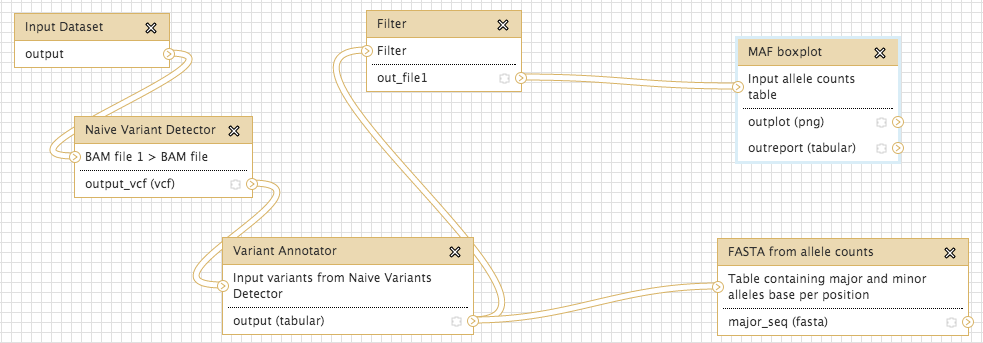
\includegraphics[width=1\textwidth]{images/galaxy-workflow-contamination.png}
%     \caption[Galaxy Workflow for Contamination estimation]{Galaxy Workflow for Contamination estimation} 
%     \label{app:galaxy-workflow}
% \end{figure}


\begin{figure}[!ht]
    \centering
    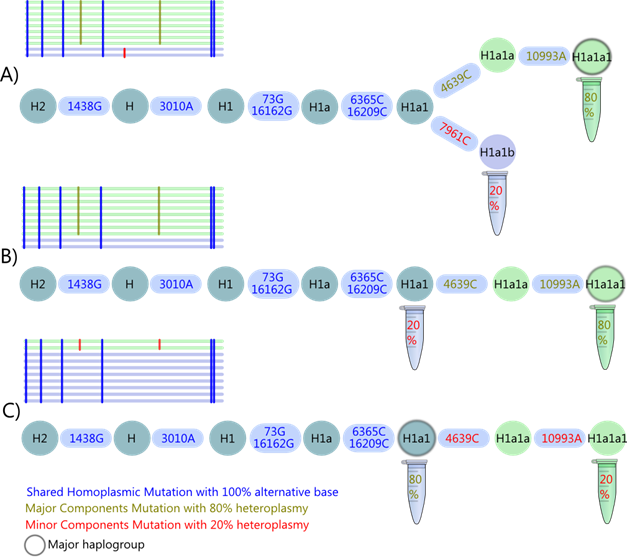
\includegraphics[width=1\textwidth]{images/heteroplasmy.png}
    \caption[Display of all possible pairwise sample contamination]{Display of all possible contaminations by pairwise comparison of major/minor haplotype within one analyzed sample. As an example a contamination level of 20\% over all reads is displayed. Shared polymorphisms of two haplotypes are presented in one branch, whereas the split into diverging branches evidences the two different lineage components (A). A mixture of two haplotypes within a single lineage but of different lineage depths (here minor H1a1 and major H1a1a1) is evidenced if no minor component can be found (B). A mixture of two haplotypes within a single lineage but of different lineage depths (here minor H1a1a1 and major H1a1) is evident if the minor components at equal levels lead to a meaningful haplogroup affiliation (C). Homoplasmic sites facilitate the identification of the branching pattern.} 
    \label{app:galaxy-boxplot}
\end{figure}

\begin{longtable}

\hline
\textbf{SampleID} & \textbf{Phy-mer} & \textbf{HaploGrep 2} & \textbf{MitoTool}           \\ \hline
KT277305          & I1a1a            & I1a1a                & I1a1a                       \\ \hline
KT277306          & I2               & I2                   & I2                          \\ \hline
KT321477          & I4a1             & I4a1                 & I4a1                        \\ \hline
KT328498          & H7h              & H7h                  & H7h                         \\ \hline
KT336633          & I1a1a            & I1a1a                & I1a1a                       \\ \hline
KT340701          & J1c2c1           & J1c2c1               & J1c2c1                      \\ \hline
KT346427          & I5, I5a          & I5                   & I5; I5a                     \\ \hline
KT359594          & J1c12            & J1c12                & J1c12                       \\ \hline
KT359595          & U7b              & U7b                  & U7b                         \\ \hline
KT359914          & U5b2a1a1         & U5b2a1a1             & U5b2a1a1                    \\ \hline
KT363958          & C1b-16311        & C1b+16311            & C1b; C1b7                   \\ \hline
KT366045          & U5a1             & U5a1                 & U5a1                        \\ \hline
KT372901          & U5a1-@16192      & U5a1+@16192          & U5a1; U5a1a; U5a1g          \\ \hline
KT372902          & U5b1e            & U5b1e                & U5b1e                       \\ \hline
KT372903          & U5b1b1           & U5b1b1               & U5b1b1                      \\ \hline
KT381969          & H5a1a            & H5a1a                & H5a1a                       \\ \hline
KT387602          & I2               & I2                   & I2                          \\ \hline
KT390700          & I4a              & I4a                  & I4a                         \\ \hline
KT390701          & H2a1             & H2a1                 & H2a1                        \\ \hline
KT424061          & U2b2             & U2b2                 & U2b2                        \\ \hline
KT427536          & H-152            & H+152                & H; H9; H46; H52; H69        \\ \hline
KT445932          & U5b3b1           & U5b3b1               & U5b3b1                      \\ \hline
KT445933          & T2a2             & T2a2                 & T2a2                        \\ \hline
KT485522          & I5a              & I5a                  & I5a4                        \\ \hline
KT625440          & H1c-152          & H1c+152              & H1c; H1c9                   \\ \hline
KT625441          & T1a2             & T1a2                 & T1a2                        \\ \hline
KT634054          & W5               & W5                   & W5                          \\ \hline
KT634229          & K1a4, K1a-150    & K1a4                 & K1a4                        \\ \hline
KT700199          & K1a4a1a2a        & K1a4a1a2a            & K1a4a1a2a                   \\ \hline
KT700200          & J2a2d            & J2a2d                & J2a2d                       \\ \hline
KT725859          & K1a11            & K1a11                & K1a11                       \\ \hline
KT756878          & L2d-16129        & L2d+16129            & L2d; L2d1                   \\ \hline
KT763050          & K1c1             & K1c1                 & K1c1                        \\ \hline
KT763051          & T2b              & T2b                  & T2b                         \\ \hline
KT764936          & U5a1b1           & U5a1b1               & U5a1b1                      \\ \hline
KT778765          & H27              & H27                  & H27                         \\ \hline
KT778766          & H7b4             & H7b4                 & H7b4                        \\ \hline
KT779554          & H7c1             & H7c1                 & H7c1                        \\ \hline
KT799550          & T1a1             & T1a1                 & T1a1                        \\ \hline
KT799551          & H44b             & H44b                 & H44b                        \\ \hline
KT799637          & H3-152           & H3+152               & H3; H3a; H3g; H3i; H3j; H3k \\ \hline
KT799679          & U6a5             & U6a5                 & U6a5                        \\ \hline
KT803044          & HV0e             & HV0e                 & HV0e                        \\ \hline
KT803045          & K1a11            & K1a11                & K1a11                       \\ \hline
KT807948          & H7c              & H7c                  & H7c                         \\ \hline
KT807955          & H5a2             & H5a2                 & H5a2                        \\ \hline
KT808880          & HV0-195          & HV0+195              & HV0; HV0b; HV0c; HV0d       \\ \hline
KT809364          & H3               & H3                   & H3                          \\ \hline
KT819292          & H3               & H3                   & H3                          \\ \hline
KT821555          & K1b2a2a          & K1b2a2a              & K1b2a2a                     \\ \hline



\end{longtable}